\documentclass[tikz,border=10pt]{standalone}
\usepackage{amsmath}
\usepackage{tikz}
\usetikzlibrary{arrows.meta, positioning, calc, shapes.geometric}

\begin{document}
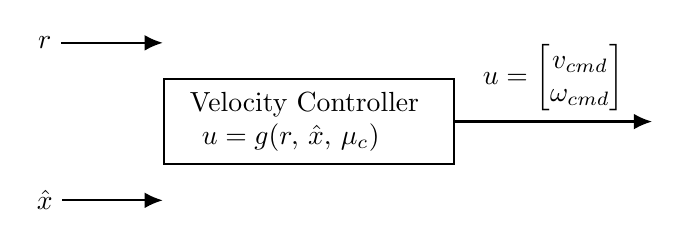
\begin{tikzpicture}[
  block/.style = {draw, thick, minimum height=3em, minimum width=6em, align=center},
  arrow/.style = {thick, -{Latex[width=2mm]}},
  node distance=2.5cm and 2.5cm
]

  % Inputs
  \node (r_in) at (0,1) {$r$};
  \node (xhat_in) at (0,-1) {$\hat{x}$};

  % Controller
  \node[block, right=1.5cm of $(r_in)!0.5!(xhat_in)$] (controller) {
    \begin{tabular}{c}
            Velocity Controller\\
      $\begin{aligned}
      u &= g(r,\,\hat{x},\,\mu_c)
       \end{aligned}$
    \end{tabular}
  };

  % Outputs
  \draw[arrow] (r_in) -- (controller.west |- r_in);
  \draw[arrow] (xhat_in) -- (controller.west |- xhat_in);
  \draw[arrow] (controller.east) -- ++(2.5,0) node[midway,above] {$u = \begin{bmatrix} v_{cmd} \\ \omega_{cmd} \end{bmatrix}$};

\end{tikzpicture}
\end{document}
